\section{Content}

\begin{frame}{Desarrollo de aplicaciones con Microprocesadores}
    \begin{itemize}
        \item Aplicaciones sencillas (fácil implementarlas mediante un bucle while, algunos timers y algunas interrupciones)
Si la complejidad de la aplicación crece, el número de temporizaciones aumenta frente al número de timers disponibles en el microprocesador y la lógica de la misma es compleja, la gestión, desarrollo y depuración de la aplicación se complican enormemente.
        \item Para simplificar esta situación se han desarrollado Sistemas Operativos “ligeros” para ser implementados en arquitecturas basadas en microprocesadores. Su utilización permite que el desarrollo de software sea más sencillo, seguro, y eficiente, redundando en un mantenimiento más sencillo del software.      
    \end{itemize}
     \centering

\end{frame}


\begin{frame}{CMSIS-RTOS}
    \begin{itemize}
      \item API C/C++ para sistemas operativos en tiempo real
      \item Diseñado para procesadores Cortex M
      \item Versión a utilizar CMSIS-RTOS2. Está se puede configurar para usar los kernels CMSIS-RTX (o keil RTX5), freeRTOS, Zephyr, embOS, Azure Thread y Micrium.
      \item En SBM usamos 2.1.3 que se basa en CMSIS v5 con RTX \href{https://arm-software.github.io/CMSIS_5/RTOS2/html/index.html}{Documentación 2.1.3}
      \item ARM ya ha lanzado la versión 2.3.0 que se basa en CMSIS V6 \href{https://arm-software.github.io/CMSIS_6/latest/RTOS2/group__CMSIS__RTOS__ThreadMgmt.html}{Documentación 2.3.0}
    \end{itemize}
    
\end{frame}

\begin{frame}{CMSIS-RTOS: Características}
    \begin{itemize}
  \item \textbf{Aplicaciones multihilo}: basada en la utilización de hilos concurrentes.
  \item Aporta mecanismos de comunicación y sincronización entre hilos.
  \item \textbf{Thread}:
    \begin{itemize}
        \item Porción de código que realiza una función concreta.
        \item Típicamente es una función con un bucle infinito y sin retorno.
        \item El RTOS permite compartir la ejecución con otros threads.
        \item 5 estados: \texttt{Running}, \texttt{Ready}, \texttt{Waiting/Blocked}, \texttt{Inactive}, \texttt{Terminated}.
    \end{itemize}
  \item \textbf{Scheduler}:
    \begin{itemize}
        \item Planificación y compartición de los recursos de CPU.
        \item Gestiona la ejecución de threads asignando tiempo (\texttt{SysTick}) de procesador a cada hilo.
    \end{itemize}
  \item \textbf{Timeslice}:
    \begin{itemize}
        \item Período de tiempo asignado a cada hilo.
        \item Múltiplo del Tick (5) generado por el \texttt{SysTick} (1ms).
    \end{itemize}
\end{itemize}

\end{frame}

\begin{frame}{CMSIS-RTOS: Planificador}
    \begin{itemize}
      \item \textbf{Pre-emptive}
          \begin{itemize}
            \item Desalojo de hilos “–prioritarios” por hilos “+prioritarios”.
          \end{itemize}
      \item \textbf{Round-Robin}
          \begin{itemize}
            \item Todos los hilos con la misma prioridad.
            \item Se ejecutan unos detrás de otros en secuencia durante un “timeslice”.
      \end{itemize}
      \item \textbf{Round-Robin Pre-emptive}
          \begin{itemize}
            \item Los hilos pueden tener distinta prioridad.
            \item Los hilos con igual prioridad se ejecutan de forma Round-Robin mientras no haya otro hilo de +prioridad en estado \texttt{READY}.
            \item Cuidado con las prioridades para no “colgar” la aplicación.
            \item Por defecto en CMSIS-RTOS - RTX.
      \end{itemize}
      \item \textbf{Cooperative Multitasking}
          \begin{itemize}
            \item Todos los hilos con igual prioridad.
            \item No Round-Robin.
            \item Cada hilo se ejecuta hasta bloquearse (pasa a \texttt{WAIT}) o hasta pasar la ejecución a otro (\texttt{yield}).
          \end{itemize}
    \end{itemize}
\end{frame}


\begin{frame}{CMSIS-RTOS: Estados en Threads}
    \begin{itemize}
        \item El planificador del SO es el encargado de gestionar la ejecución de un thread
        \item Estados de un thread:
       \begin{itemize}
          \item \textbf{RUNNING}: thread actualmente en ejecución.
          \item \textbf{READY}: threads preparados para ser ejecutados. Una vez que la tarea que se está ejecutando ha consumido su \textit{timeslice}, la siguiente tarea con máxima prioridad pasa a \textbf{RUNNING}.
          \item \textbf{BLOCKED/WAITING}: threads esperando la ocurrencia de algún evento.
          \item \textbf{TERMINATED}: threads terminados pero sin liberar recursos.
          \item \textbf{INACTIVE}: threads no creados o terminados. No consumen ningún recurso.
        \end{itemize}
    \end{itemize}
    
\end{frame}

\begin{frame}[fragile]{Thread in Keil Microvision}
    \begin{minted}[fontsize=\scriptsize, bgcolor=blue!5]{c}
    #include "cmsis_os2.h"
    
    osThreadId_t tid_thread; // tid_thread identifica al thread.Se usará en funciones específicas del RTOS
    ...
    
    tid_Thread = osThreadNew(Thread, NULL, NULL);
    if (tid_Thread == NULL) {
        return(-1);
    }


    void Thread (void *argument){
        // inserte el código que solo quiera que se ejecute una vez
        while(1){
        // inserte el código que quiera que se ejecute continuamente
        
        }
        // nunca se llega a este punto en este ejemplo
    
    }
    \end{minted}
    \begin{itemize}
        \item Es altamente aconsejable crear un fichero de cabecera donde se deberán declarar la función de inicio para poder ser utilizados por otros módulos del software

    \end{itemize}
\end{frame}

\begin{frame}[fragile]{Implementación de aplicaciones con Threads}
    \begin{columns}
        \begin{column}{0.50\textwidth}
            \begin{minted}[fontsize=\scriptsize, bgcolor=blue!5]{c}
// Fichero con thread ThDisplay.c
#include "cmsis_os2.h"
#include "ThDisplay.h"

osThreadId_t tid_ThDisplay; 
...

tid_ThDisplay = osThreadNew(ThDisplay, 
                NULL, NULL);
if (tid_ThDisplay == NULL) {
    return(-1);
}


void ThDisplay (void *argument){
    int ciclo=0;
    Init_display();
    while(1){
    .....
    
    }
   

}
            \end{minted}
        \end{column}
    \begin{column}{0.50\textwidth}
        \begin{minted}[fontsize=\scriptsize, bgcolor=blue!5]{c}
        // Fichero main.c
        #include "ThDisplay.h"
        int main(void){
            int status=0;
            HAL_Init();
            SystemClock_Config();
            SystemCoreClockUpdate();
        #ifdef RTE_CMSIS_RTOS2
            oskernelInitilize();
            status|= Init_ThDisplay();
            osKernelStart();
        #endif
        }
        \end{minted}
        \begin{minted}[fontsize=\scriptsize, bgcolor=blue!5]{c}
        // Fichero de cabecera  ThDisplay.h    
        #include "stm32f4xx_hal.h"
        
        #ifndef __THDISPLAY__H
        #define __THDISPLAY__H
            #define S_PINTA  0x0001U
            int Init_ThDisplay(void);
        #endif
        
        \end{minted}
    \end{column}
    \end{columns}
    \begin{itemize}
        \item Es altamente aconsejable crear un fichero de cabecera donde se deberán declarar la función de inicio para poder ser utilizados por otros módulos del software

    \end{itemize}
\end{frame}

\begin{frame}{CMSIS RTOs Sincronización}
    \begin{columns}
        \begin{column}{0.50\textwidth}
            \begin{itemize}
                \item Una aplicación usará múltiples threads y recursos que hay que sincronizar
                \item ¿Cúal es el problema?
                    \begin{itemize}
                        \item Varios threads se ejecutan concurrentemente y quieren usar el mismo recurso compartido que puedes ser software o hardware
                        \item Hay que garantizar el uso secuencial del recurso compartido
                    \end{itemize}
                \item ¿Cuál es la solución?
                \begin{itemize}
                    \item Usar recursos como eventos, flags, colas, semáforos, etc
                    \item CMSIS-RTOS V2 implementa una API con estos recursos
                \end{itemize}
            \end{itemize}    
        \end{column}
        \begin{column}{0.50\textwidth}
            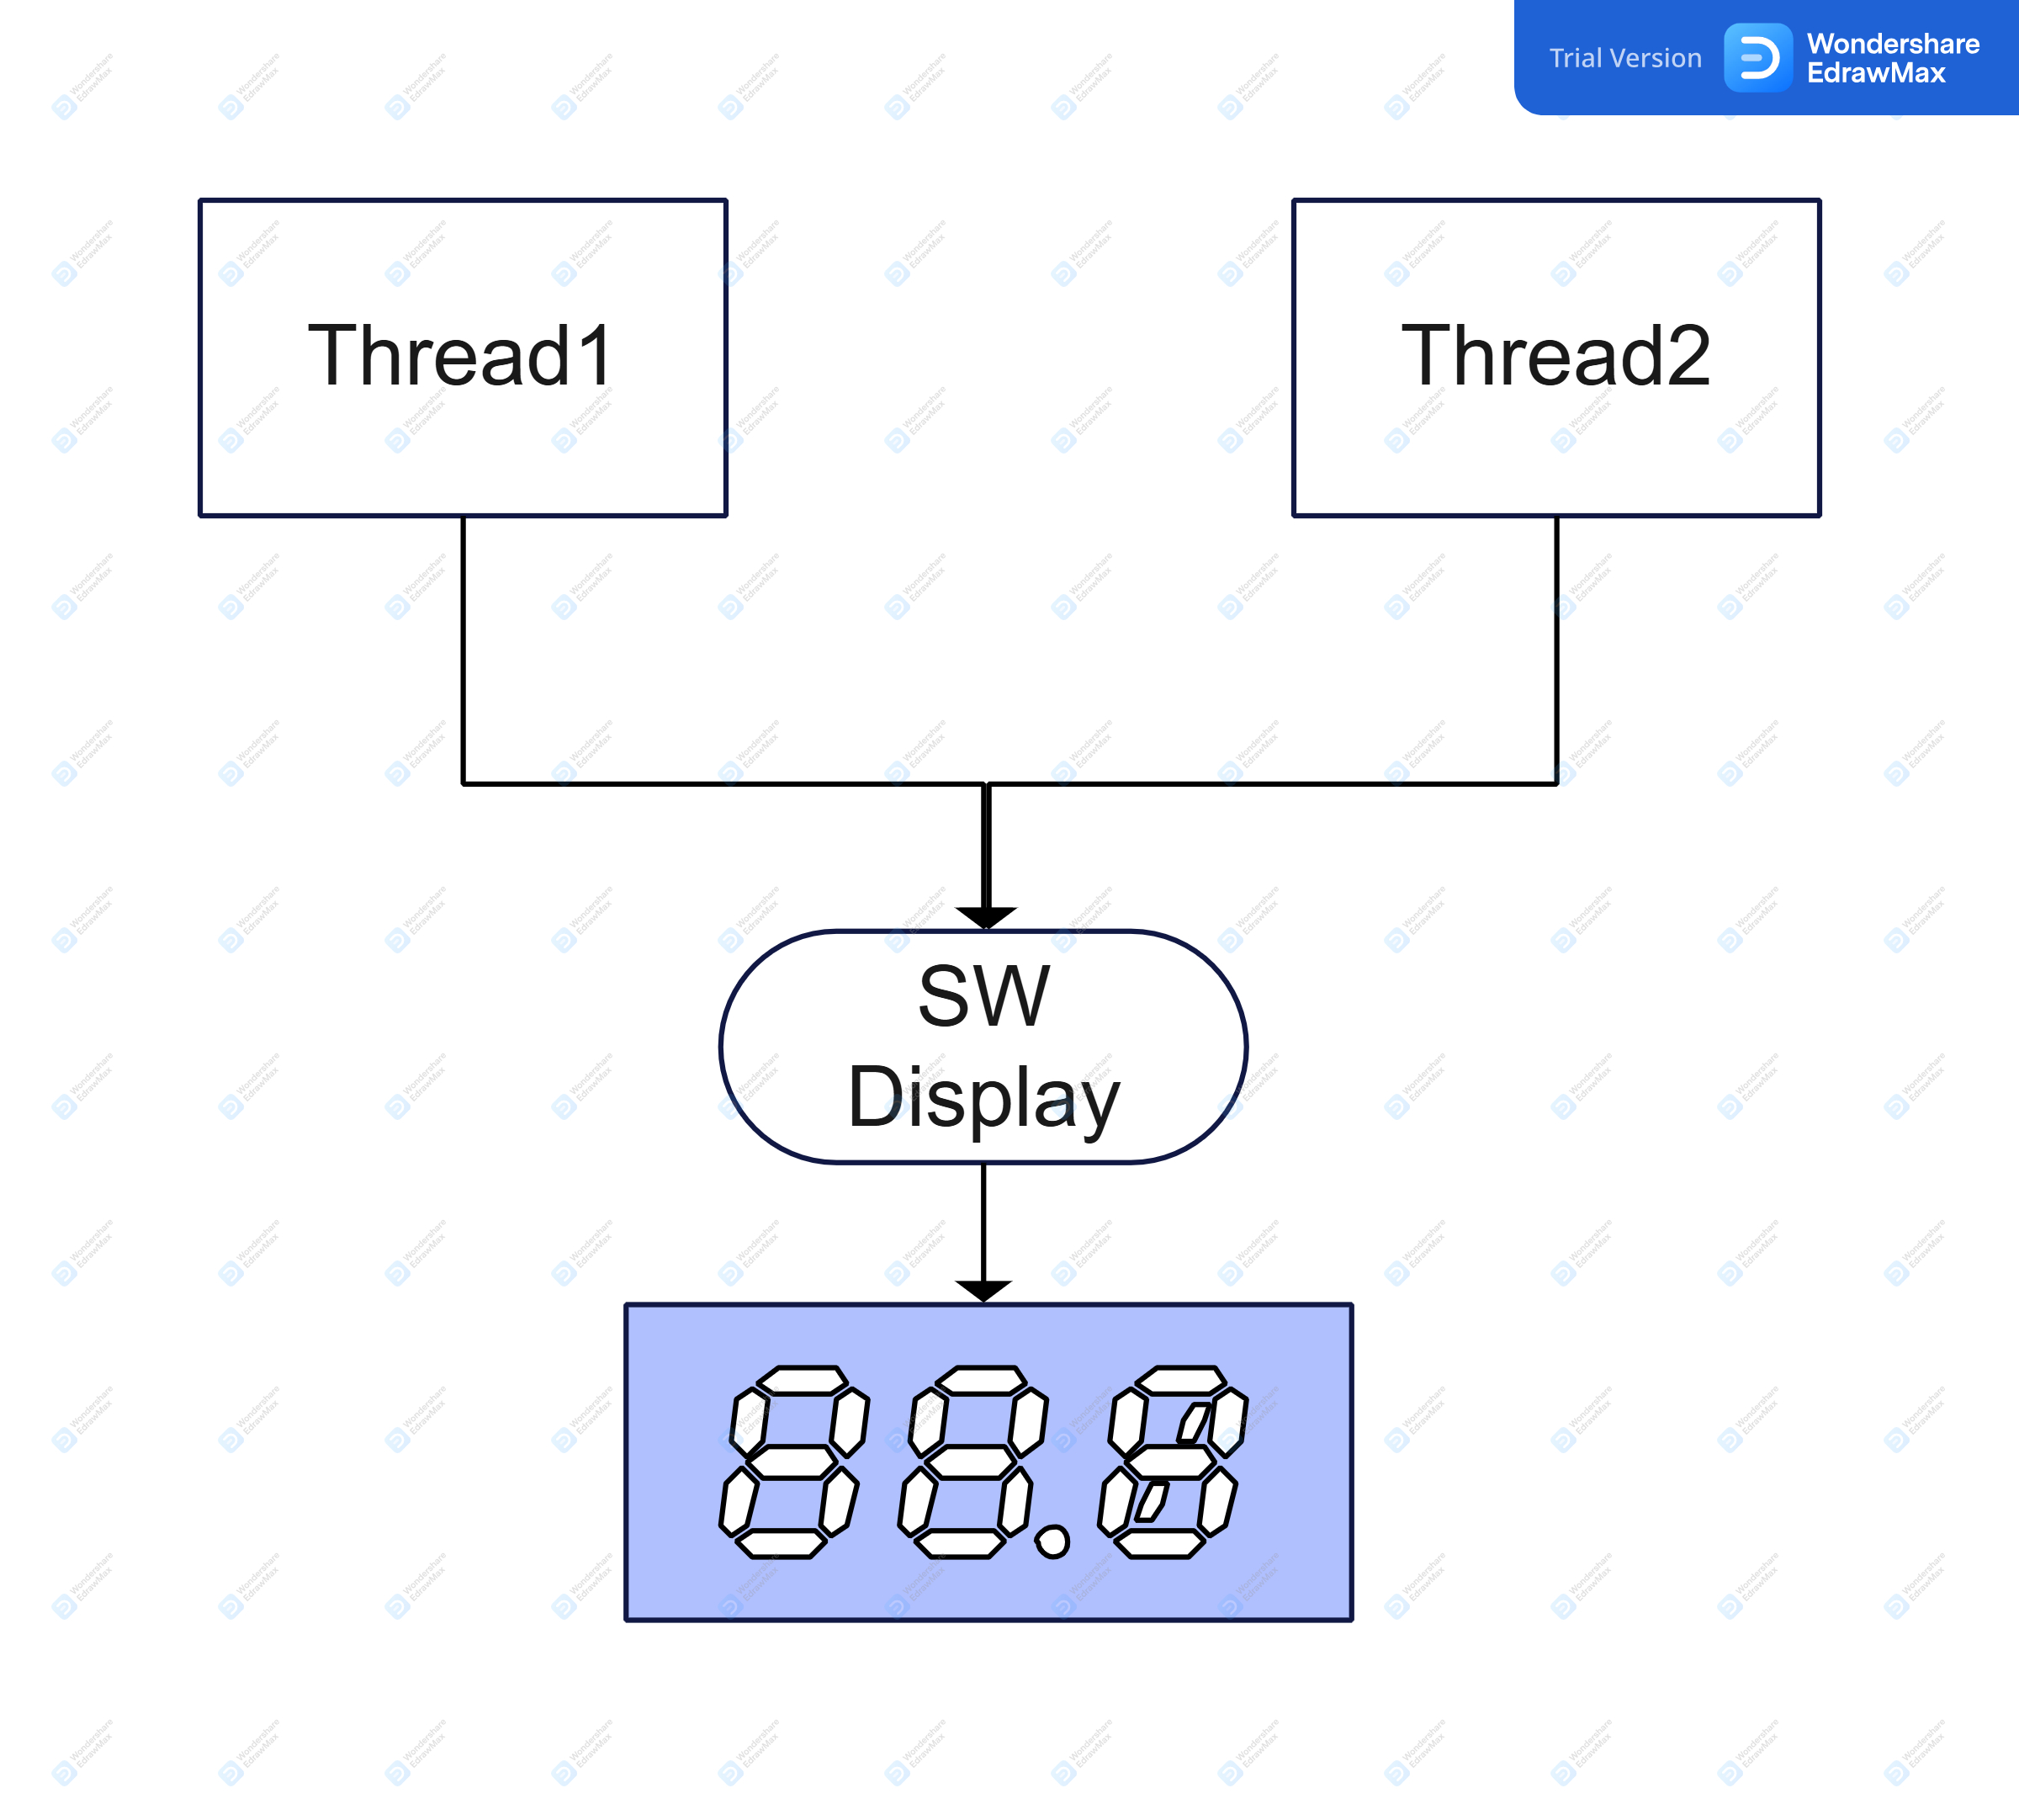
\includegraphics[scale=0.05]{presentation/threads.jpg}
        \end{column}
    \end{columns}
\end{frame}
\begin{frame}{CMSIS RTOs Sincronización}
    \begin{columns}
        \begin{column}{0.50\textwidth}
            \begin{itemize}
                \item Una posible solución. Se añade una cola gestionada por el Sistema Operativo
                \item Existe un thread que lee los mensajes que llegan a a la cola para enviarlos al display 
                \item Cada thread que quiere enviar un mensaje al LCD escribe en la cola
            \end{itemize}    
        \end{column}
        \begin{column}{0.50\textwidth}
            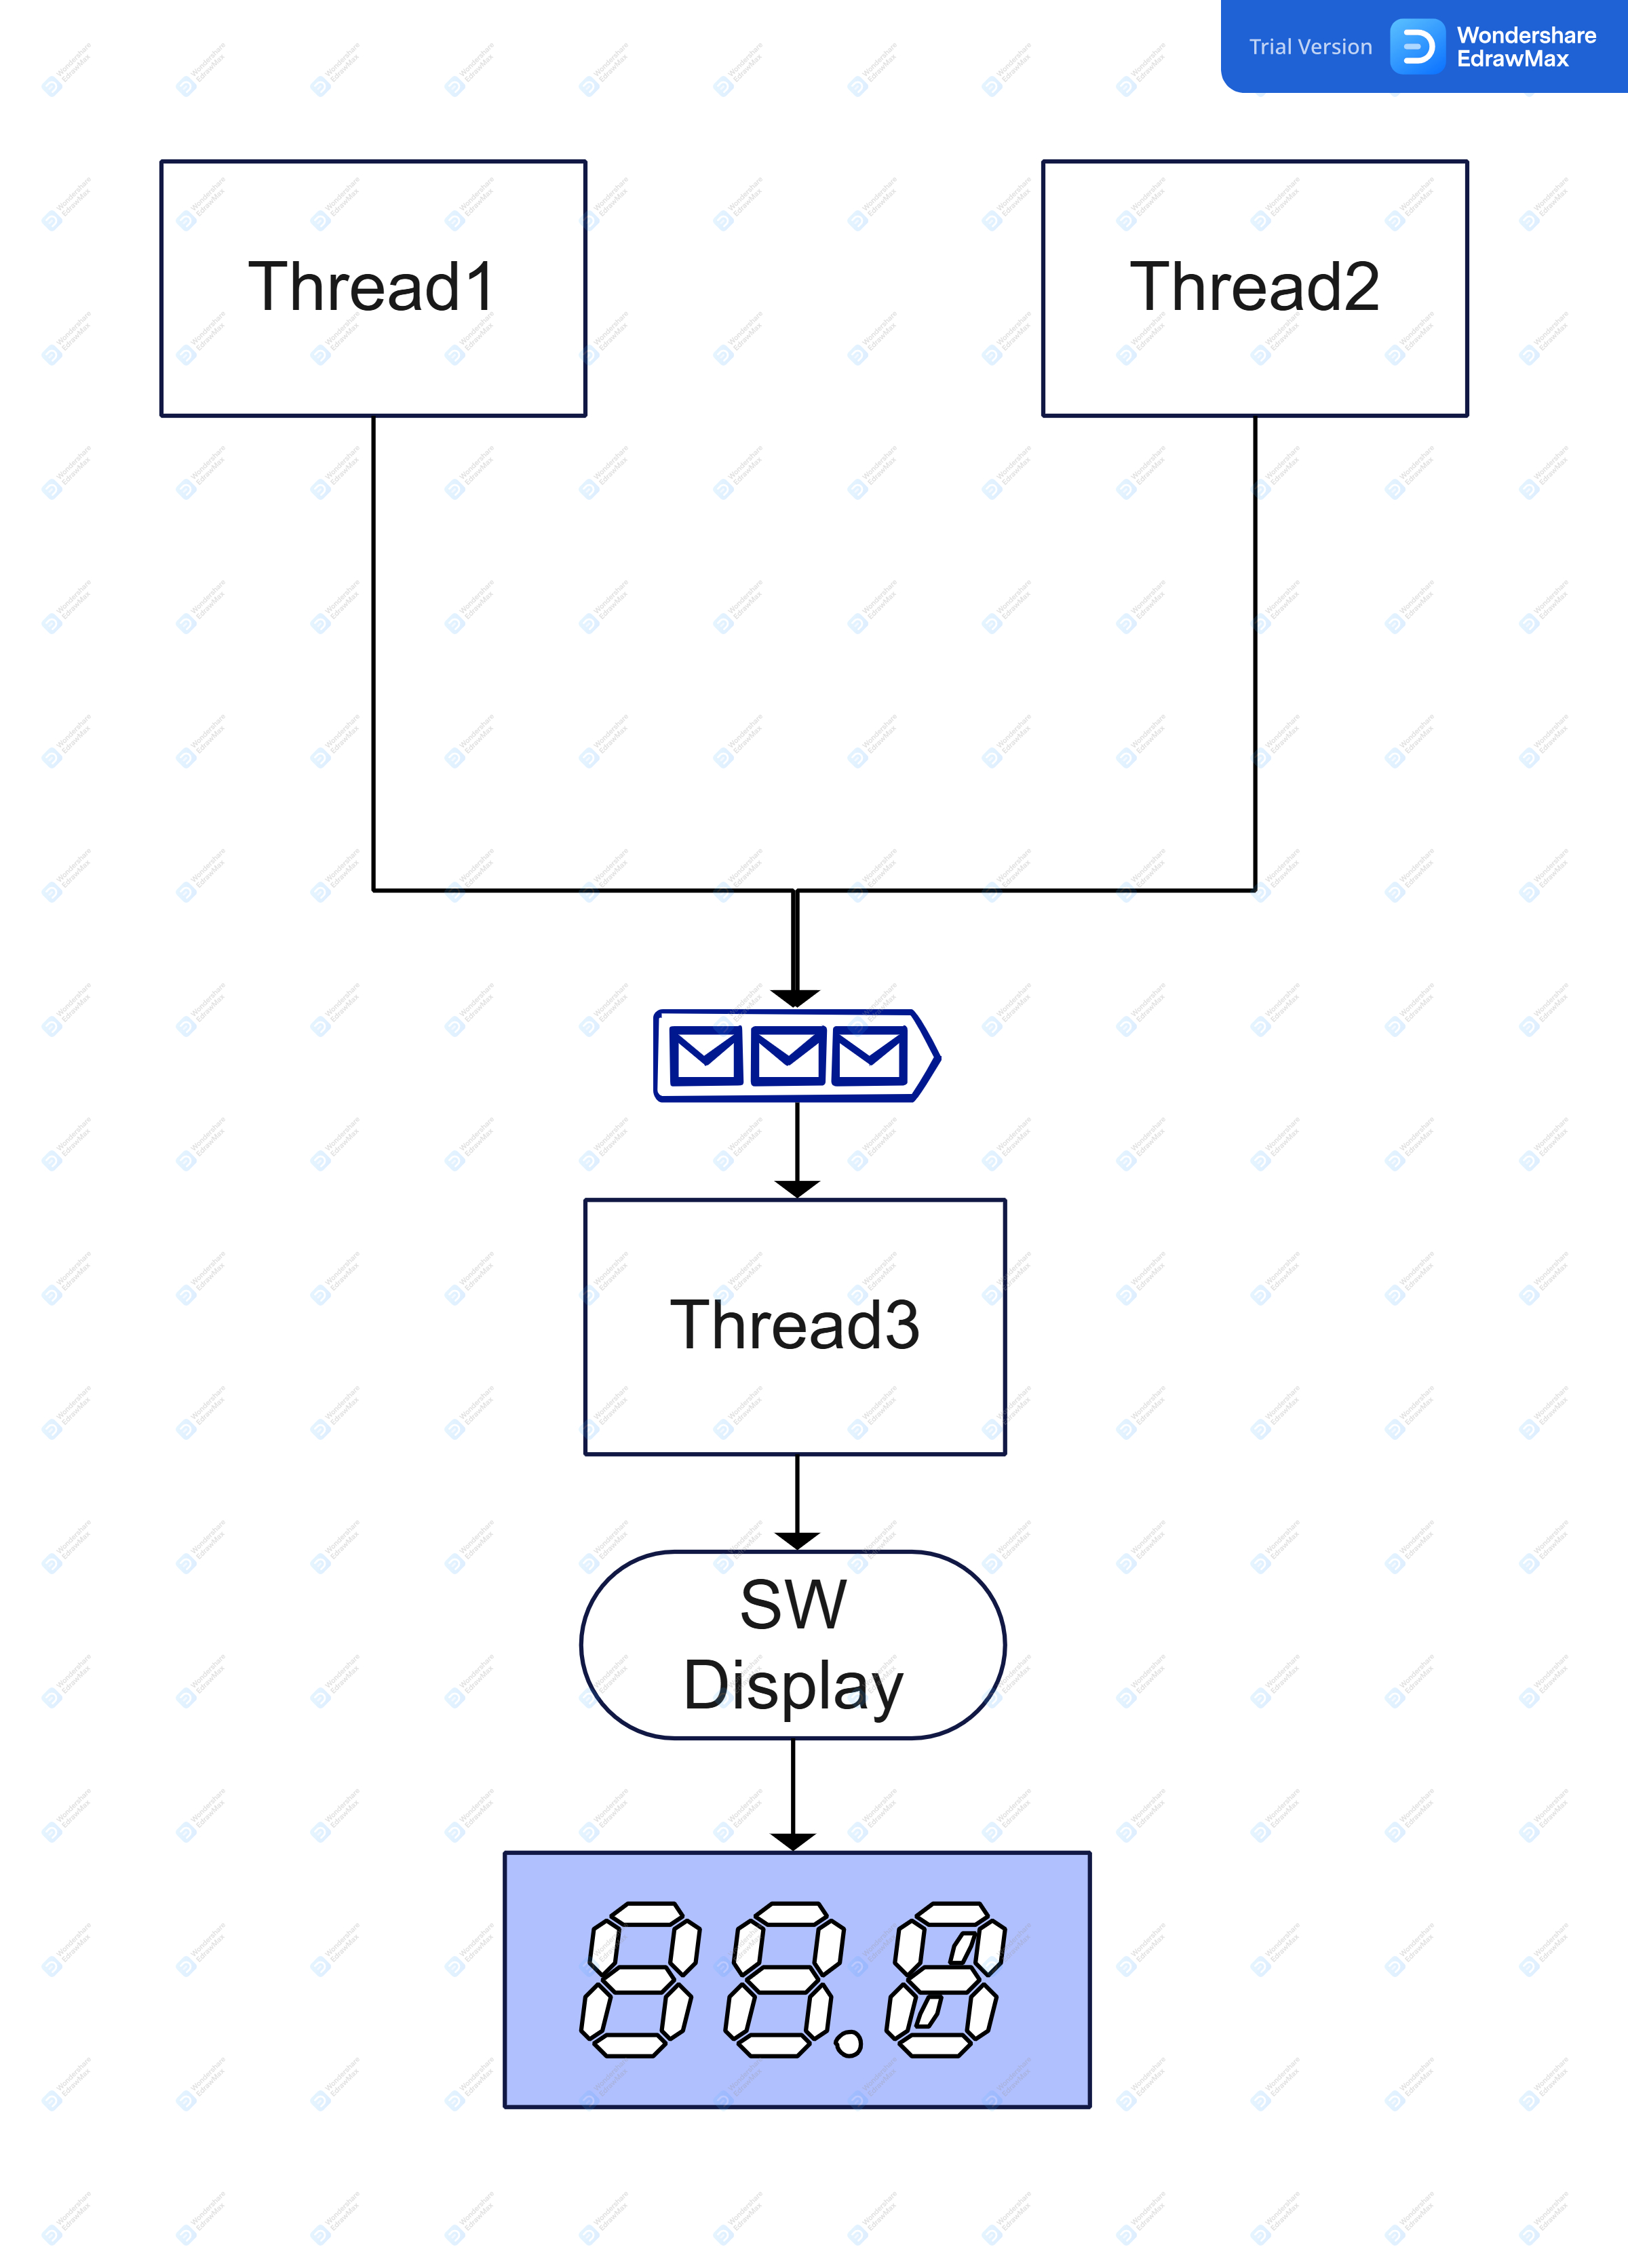
\includegraphics[scale=0.05]{presentation/threads-sync.jpg}
        \end{column}
    \end{columns}
\end{frame}

\begin{frame}[fragile]{Sincronización con Thread Flags}
      \begin{itemize}
          \item \textbf{Problema:} La tarea 1 genera periódicamente eventos/datos (1s). Queremos que la tarea 2 solo se ejecute cuando haya un dato disponible y que no consuma CPU mientras tanto.
      \end{itemize}
      \begin{columns}
            \begin{column}{0.50\textwidth}
                \begin{itemize}
                    \item[]                      
                    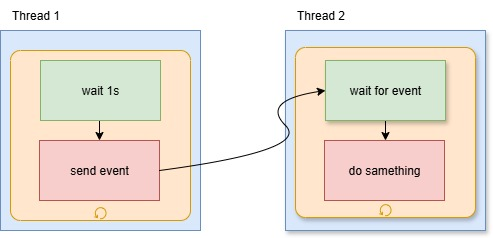
\includegraphics[scale=0.25]{presentation/flags.jpg}
                    \item El Thread 2 pasa al estado de \textbf{Waiting} hasta que el Thread 1 active el flag.
                    \item Cuando el flag o el conjunto de flags son activados el hilo pasa al estaddo \textbf{Ready}
                \end{itemize}
            \end{column}
            \begin{column}{0.50\textwidth}
             \begin{minted}[fontsize=\scriptsize, bgcolor=blue!5]{c}
void Thread1 (void *argument){
    while(1){
    osdelay(1000);
    osThreadFlagSet(tid_thread2, 0x0001);
    }
}

void Thread2 (void *argument){
    while(1){
    status = osThreadFlagWait(0x0001,
             osFlagsWaitAny, 
             osWaitForever);
    //
    }
}
             \end{minted}
             
            \end{column}
     \end{columns}
\end{frame}

\begin{frame}[fragile]{CMSIS RTOs Thead Flags}

    \begin{itemize}
        \item []
         \begin{minted}[fontsize=\scriptsize, bgcolor=blue!5]{c}
uint32_t osThreadFlagSet(osThreadId_t thread_id, uint32_t flags)
/* Activa el flag especificado de una tarea activa
Se puede llamar desde una interrupción */

         \end{minted}
         \begin{minted}[fontsize=\scriptsize, bgcolor=blue!5]{c}
uint32_t osThreadFlagClear(osThreadId_t thread_id, uint32_t signals)
/* Borra el flag especificado de una tarea activa
No se puede llamar desde una interrupción*/

         \end{minted}
         \begin{minted}[fontsize=\scriptsize, bgcolor=blue!5]{c}
uint32_t osThreadFlagsWait(uint32_t flags, uint32_t options, uint32_t timeout)
/* Espera a uno o más Flags para continuar la ejecución
No se puede llamar desde una interrupción */

         \end{minted}
         \begin{minted}[fontsize=\scriptsize, bgcolor=blue!5]{c}
uint32_t osThreadFlagGet(void)
/* Retorna los flags del thread en ejecución 
No se puede llamar desde una interrupción */

         \end{minted}      
         \item[] \href{https://arm-software.github.io/CMSIS_5/RTOS2/html/group__CMSIS__RTOS__ThreadFlagsMgmt.html}{\colorbox{BurntOrange}{CMSIS RTOS V2 Thread Flags reference}}
    \end{itemize}     
\end{frame}